\documentclass[article]{ajs}

%%%%%%%%%%%%%%%%%%%%%%%%%%%%%%
%% declarations for jss.cls %%%%%%%%%%%%%%%%%%%%%%%%%%%%%%%%%%%%%%%%%%
%%%%%%%%%%%%%%%%%%%%%%%%%%%%%%

%% additional packages
\usepackage{wrapfig}
\usepackage{graphicx}
\usepackage{subcaption}

%% definitions of entities in formulae
% Model:
\newcommand{\nDomains}{D}
\newcommand{\indexDomain}{i}
\newcommand{\directStat}{y}
\newcommand{\directStatIndexed}{y_{\indexDomain}}
\newcommand{\trueStat}{\mu}
\newcommand{\trueStatIndexed}{\mu_{\indexDomain}}
\newcommand{\indexUnit}{j}
\newcommand{\nUnitIndexed}{n_\indexDomain}

% Sampling-Error
\newcommand{\samplingError}{e}
\newcommand{\samplingErrorIndexed}{e_{\indexDomain}}
\newcommand{\samplingErrorUnitIndexed}{e_{\indexDomain\indexUnit}}
\newcommand{\samplingVariance}{\sigma_e^2}
\newcommand{\samplingVarianceIndexed}{\sigma_{e, i}^2}
\newcommand{\samplingSD}{\sigma_e}

% Uni Error
\newcommand{\unitError}{e}

% Random Effects
\newcommand{\randomEffectIndexed}{v_{\indexDomain}}
\newcommand{\randomEffect}{v}
\newcommand{\randomEffectVariance}{\sigma_v^2}
\newcommand{\randomEffectSD}{\sigma_v}
\newcommand{\RandomEffect}{\mathbf{v}}

% Regressors
\newcommand{\xArea}{x_{\indexDomain}}
\newcommand{\xUnit}{x_{\indexDomain\indexUnit}}
\newcommand{\X}{\mathbf{X}}
\newcommand{\indexRegressor}{p}
\newcommand{\nRegressor}{P}


%% almost as usual
\author{Sebastian Warnholz\\ Freie Universit\"at Berlin \And 
        Timo Schmid \\ Freie Universit\"at Berlin}
\title{Simulation Tools for Small Area Estimation: Introducing the \proglang{R}-package \proglang{saeSim}}

%% for pretty printing and a nice hypersummary also set:
\Plainauthor{Sebastian Warnholz, Timo Schmid} %% comma-separated
\Plaintitle{Simulation Tools for Small Area Estimation: Introducing the R-package saeSim} %% without formatting
\Shorttitle{Simulation Tools for Small Area Estimation} %% a short title (if necessary)

%% an abstract and keywords
\Abstract{
The demand for reliable regional estimates from sample surveys has been substantially grown over the last decades. Small area estimation provides statistical methods to produce reliable predictions when the sample sizes in regions are too small to apply direct estimators. Model- and design-based simulations are used to gain insights into the quality of the introduced methods. In this article we present a framework which may help to guarantee the reproducibility of simulation studies in articles and during research. The introduced \proglang{R}-package \proglang{saeSim} is adjusted to provide a simulation environment for the special case of small area estimation. The package may allow the prospective researcher during the research process to produce simulation studies with a minimal effort of coding.   
}

\Keywords{Package, \proglang{R}, reproducible research, simulation study, small area estimation}
\Plainkeywords{package, R, reproducible research, simulation, small area estimation} %% without formatting
%% at least one keyword must be supplied

%% publication information
%% NOTE: Typically, this can be left commented and will be filled out by the technical editor
%% \Volume{50}
%% \Issue{9}
%% \Month{June}
%% \Year{2012}
%% \Submitdate{2012-06-04}
%% \Acceptdate{2012-06-04}
%% \setcounter{page}{1}
\Pages{1--xx}

%% The address of (at least) one author should be given
%% in the following format:
\Address{
  Timo Schmid\\
  Department of Economics\\
  Freie Universit\"at Berlin\\
  D-14195 Berlin, Germany\\
  E-mail: \email{Timo.Schmid@fu-berlin.de}\\
  URL: \url{http://www.wiwiss.fu-berlin.de/fachbereich/vwl/Schmid}\\
  
  Sebastian Warnholz\\
  Department of Economics\\
  Freie Universit\"at Berlin\\
  D-14195 Berlin, Germany\\
  E-mail: \email{Sebastian.Warnholz@fu-berlin.de}\\
  URL: \url{http://www.wiwiss.fu-berlin.de/fachbereich/vwl/Schmid/Team/Warnholz.html}
}


%% It is also possible to add a telephone and fax number
%% before the e-mail in the following format:
%% Telephone: +43/512/507-7103
%% Fax: +43/512/507-2851

%% for those who use Sweave please include the following line (with % symbols):
%% need no \usepackage{Sweave.sty}

%% end of declarations %%%%%%%%%%%%%%%%%%%%%%%%%%%%%%%%%%%%%%%%%%%%%%%


\begin{document}
%
%% include your article here, just as usual
%
% R CMD Sweave %.Rnw
% Loading (and installing) necessary packages.
%
\section{Introduction}
The demand for reliable small area statistics from sample surveys has been substantially grown over the last decades due to their use in public and private sectors. In this paper we present a framework for simulation studies inside the field of small area estimation. This tool might be useful for the prospective researcher or data analyst to provide reproducible research.

Reproducible research has become a widely discussed topic. In the field of statistics many open-source tools like the \proglang{R}-language \citep{r14} and \LaTeX, dynamic reporting packages like \proglang{knitr} \citep{yihui13}, \proglang{sweave} \citep{leisch02} and more recently \proglang{rmarkdown} \citep{allaire14}, make the integration of text and source code for statistical analysis possible. Publishing source code and data alongside research results draws special attention to authoring the analysis. However, the requirements for source code are different from the written words in the article itself. 

\begin{quote}
\textit{Instead of imagining that our main task is to instruct a computer what to do, let us concentrate rather on explaining to human beings what we want a computer to do.} \cite[p.99]{knuth92} 
\end{quote} 

Next to the combination of text and source code, reproducible research aims that the full output of the academic research, which is the paper combined with the full computational environment like data and source code, is available. However, real data is often very sensitive and governed by strict confidentiality rules. Synthetic data generation mechanisms \citep{Kol11} can be used to provide safe data which is publicly available to enable the community to reproduce the analysis and results. \cite{Bur14} interpreted this as an open research philosophy. Such synthetic data sets can be used to test newly proposed statistical methods in a close-to-reality framework. 
%This may provide valuable insights about the quality of the introduced methods in a controlled environment under different scenarios. 
In general, simulation studies in statistics can be divided into two concepts:
%
\begin{itemize}
\item Design-based: The simulation study is based on true or synthetic data of a fixed population. Then, samples are selected repeatedly from the underlying finite population and different estimation methods are applied in each replication. The obtained estimates are compared to the true values of the population, for instance, in terms of relative bias (RB) or relative root mean squared error (RRMSE).
\item Model-based: The simulation study uses data drawn from certain distributions. In each iteration, the population is generated from a model and a sample is selected according to a specific sampling scheme. The sample is used to estimate the quantity of interest and quality measures (like RB and RRMSE) are derived.  
\end{itemize}
Further discussion regarding model- and design-based simulations is available in \cite{Mue03}, \cite{Sal10} or \cite{Alf10}.

\cite{Alf10} provide the \proglang{R}-package \proglang{simFrame} which helps to conduct simulation studies in a reproducible environment. It includes a wide range of different features (like data generation, sampling schemes, outlier contamination mechanisms and missing values) to conduct simulation studies. \proglang{simFrame} was originally developed for simulations in the context of survey statistics but is now designed to be as general as possible \citep[cf.][]{Alf10}.

Survey statistics are used, for example, in order to deliver specific indicators as a basis for economic and political decision processes. Especially regional or group-specific comparisons are of interest \citep[cf.][]{Sch13}. Surveys which shall provide the sufficient data for these regional indicators, however, are generally designed for larger areas (NUTS 1-2 level). Hence, sample information on more detailed levels, like NUTS3, is hardly available so that classical estimation methods (direct estimators) may lead to high variances of the estimates \citep[cf.][]{Gho94}. In this case, small area estimation methods may reveal highly improved results for the target estimates. Small area estimation has become more and more attractive over the last decade: 

\begin{quote}
\textit{In 2002, small area estimation (SAE) was flourishing both in research and applications, but my own feeling then was that the topic has been more or less exhausted in terms of research and that it will just turn into a routine application in sample survey practice. As the past 9 years show, I was completely wrong; not only is the research in this area accelerating, but it now involves some of the best known statisticians...} \cite{pfeffermann13} 
\end{quote} 

However, simulation studies in the context of small area estimation is often presented very briefly. Thus, there is a need to have a suited framework to guarantee the reproducibility of analysis. To the best of our knowledge, there is not any \proglang{R}-package or framework adjusted for the special case of small area estimation which provides a simulation environment.

The aim of this article is to introduce a new \proglang{R}-package, \proglang{saeSim}, which supports the process of making simulation studies in the field of small area estimation reproducible. To be more precise, the package has three main objectives: First, provide tools for data generation. Second, unify the process of simulation studies. Third, make the source-code of simulation studies available, such that it supports the conducted research in a transparent manner.

The paper is organised as follows. In Section \ref{sec:SAE} we give a short introduction to small area estimation focusing mainly on unit-level \citep{battese88} and area-level models \citep{fay79}. Section \ref{sec:framework} introduces a framework for simulation studies and how it is supported by the  \proglang{R}-package \proglang{saeSim}. To illustrate some of the features of the package we present a model- and design-based simulation study in Section \ref{sec:caseStudy}. We conclude the paper in Section \ref{sec:outlook} by summarising the main findings and by providing some avenues for further research.


\section{Small area estimation}
\label{sec:SAE}

The objective of small area estimation is to produce reliable statistics (means, quantiles, proportions, etc.) for domains where less or no sampled units are available. Groups may be areas or other entities, for example defined by socio-economic characteristics. The demand for such estimators is rising as they are used for fund allocation, educational and health programs \citep{pfeffermann13}. As direct estimation of such statistics are considered to be unreliable (with respect to MSE), methods in small area estimation try to improve the domain predictions by borrowing strength from neighboured or \textit{similar} domains. This can be achieved by using additional information from census data or registers to assist the prediction for non-sampled domains or domains with small sample sizes. 

For the purpose of this article we will introduce two basic models frequently used in small area estimation, the unit-level model introduced by \cite{battese88} and the area-level model introduced by \cite{fay79}. The unit level model \citep{battese88} can be expressed as:
\begin{eqnarray}
	 y_{\indexDomain\indexUnit} =& \xUnit^\top\beta + \randomEffectIndexed + \samplingErrorUnitIndexed \nonumber \\
	\randomEffectIndexed \stackrel{iid}{\sim}& N(0, \randomEffectVariance)  \nonumber \\
	\samplingErrorUnitIndexed \stackrel{iid}{\sim}& N(0, \samplingVariance) \nonumber,
\end{eqnarray}

where $\indexDomain = 1, \dots, \nDomains$ and $\indexUnit = 1, \dots, \nUnitIndexed$. The population of size $N$ is divided into $D$ non-overlapping small areas of sizes $N_i$ and into $n$ sampled and $N-n$ non-sampled units, denoted by $s$ and $r$ respectively. $y_{\indexDomain\indexUnit}$ is the dependent variable for domain $\indexDomain$ and unit $\indexUnit$, and $\xUnit$ are the corresponding auxiliary information for that unit. Furthermore $\randomEffect$ and $\samplingError$ are independent. Let $\hat{\beta}$ denote the best linear unbiased estimator (BLUE) of $\beta$ and $\hat{\randomEffectIndexed}$ the best linear unbiased predictor (BLUP) of $\randomEffectIndexed$ (cf.\ \citealp{Hen50} or \citealp{Sea71}). The empirical best linear unbiased predictor (EBLUP) for the mean in small area $i$ in the Battese-Harter-Fuller model is then given by
\begin{eqnarray}\label{BHFEBLUP}\hat{\overline{y}}_i^{BHF}&=&N_i^{-1}\Big\{\sum_{j\in s_i}y_{ij}+\sum_{j\in r_i}(\xUnit^\top\hat{{\beta}}+\hat{\randomEffectIndexed})\Big\}.
\end{eqnarray}

Due to reasons of confidentiality unit-level information is not always available. Instead only aggregates for the domains or direct estimators may be supplied. In this case the feasible direct estimates are known to be unreliable in the case of small sample sizes. Here area-level models can be valuable. The area-level model introduced by \cite{fay79} is build on a sampling model:
%
\[\directStat_{\indexDomain} = \trueStat_{\indexDomain} + \samplingError_{\indexDomain},\]
%
where $\directStat_{\indexDomain}$ is a direct estimator of a statistic of interest $\trueStat_{\indexDomain}$ for an area $\indexDomain$. The sampling error $\samplingError_{\indexDomain}$ is assumed to be independent and normally distributed with known variances $\samplingVarianceIndexed$, i.e. $\samplingError_{\indexDomain}|\trueStat_{\indexDomain} \sim \mathit{N}(0, \samplingVarianceIndexed)$. The model assumes a linear relationship between the true area statistic $\trueStat_{\indexDomain}$ and some auxiliary variables $\xArea$:
%
\[\trueStat_{\indexDomain} = \xArea^\top \beta + \randomEffectIndexed,\] 
%
with $\indexDomain=1,\dots, \nDomains$. 
%Note that $\xArea$ is a vector containing area-level (aggregated) information for $\nRegressor$ variables and $\beta$ is a vector ($1\times \nRegressor$) of regression coefficients describing the (linear) relationship. 
The model errors $\randomEffectIndexed$ are assumed to be independent and normally distributed, i.e. $\randomEffectIndexed \sim \mathit{N}(0, \randomEffectVariance)$. Furthermore $\samplingErrorIndexed$ and $\randomEffectIndexed$ are assumed to be independent. Combining the sampling and linking model leads to:
\begin{equation}
\label{eq:FH}
\directStatIndexed = \xArea^\top \beta + \randomEffectIndexed + \samplingErrorIndexed.
\end{equation} 
%
The Fay-Herriot (FH) model in (\ref{eq:FH}) is effectively a random-intercept model where the distribution of the error term $\samplingErrorIndexed$ is heterogeneous and known. The EBLUP of the small area mean in the FH model is given by 
\begin{eqnarray}\label{FHEBLUP}\hat{\overline{y}}_i^{FH}&=&\xArea^\top \hat{\beta} + \hat{\randomEffectIndexed}.
\end{eqnarray}

\section{A simulation framework}
\label{sec:framework}
%
%% flow-diagram
\begin{wrapfigure}{R}{0.5\textwidth}
\begin{center}
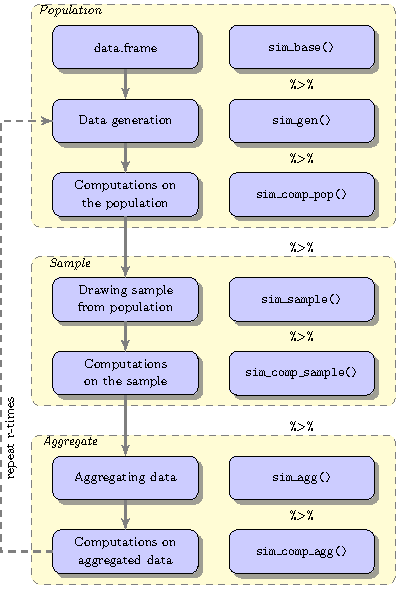
\includegraphics[width=0.5\textwidth]{flowdiagram}
\end{center}
\caption{\label{fig:flowdiagram}Process of simulation. Left column are the steps in a simulation. Right column are the corresponding function names to represent those steps in \proglang{R}.} 
\end{wrapfigure}
%
In this section we will present the simulation framework implemented in \proglang{saeSim}. The framework relies strongly on the idea to describe a simulation as a process of data manipulation. Independent of simulation studies, \cite{wickham14a} and \cite{wickham14b} strongly promote this idea by providing tools for cleaning and transforming data. In those frameworks every defined function takes a \proglang{data.frame} as input and returns it modified. This leads to a natural connection between all defined functions as the result of one function can be directly passed to the next as an argument. The symbioses of these packages with the pipe operator (\proglang{\%>\%}) from the package \proglang{magrittr} \citep{bache14} only emphasises the process of data manipulation. To avoid nested function calls the operator can be used to improve the readability as expressions can be read from left to right (cf. Section \ref{sec:caseStudy}).

In \proglang{saeSim} we extend this approach to simulation studies in the field of small area estimation. The main focus lies on the description of a simulation as a process of data manipulation. Each step in this process can be defined as a self contained component (function) and thus can be easily replaced, extended and most importantly reused. Before we go into details of the functionality of the package we discuss the process behind simulation studies and how \proglang{saeSim} maps this process into \proglang{R}.

Simulation studies in small area estimation address three different levels, the population, the sample and data on aggregated level. Figure \ref{fig:flowdiagram} illustrates these levels. The left column describes the steps of data manipulation, the right column presents the function names to define the corresponding steps. The \textbf{population-level} defines the data on which a study is conducted and may be a true population, synthetic population data or randomly generated variates from a model. We see two different point of views to define a population: Firstly, \textit{design-based} simulations, which means that a simulation study is based on true or synthetic data of \textit{one} population. Secondly, \textit{model-based} simulations, which have changing random populations drawn from a model.

The scope of this article is not to promote any of those viewpoints, we just want to incorporate the different simulation concepts in a common framework. The \textit{base} (first component in Figure \ref{fig:flowdiagram}) of a simulation study is a data table, the question is, if this data is \textit{fixed} or \textit{random} over simulations. Or from a more technical point of view, is the data generation (the second step in Figure \ref{fig:flowdiagram}) repeated in each simulation run or omitted. Depending on the choice of a fixed or random population it is necessary to recompute the population domain-statistics like domain means and variances, or other statistics of interest (third component in Figure \ref{fig:flowdiagram}).

The \textbf{sample-level} is necessary when domain predictions are conducted for unit-level models. Independently of how the population is treated, fixed or random, this phase consists of two steps: Firstly, draw a sample according to a specific sampling scheme. Secondly, conduct computations on the samples (fourth and fifth component in Figure \ref{fig:flowdiagram}). Given a sample, small area methods are applied. Of interest are, for instance, estimated model parameters, domain predictions or measures of uncertainty (MSE) for the estimates.

As the sample-level is necessary when unit-level models are applied, the \textbf{aggregate-level} is conducted when area-level models are applied (the seventh and last component in Figure \ref{fig:flowdiagram}). Area-level models in small area estimation typically only use information available for domains (in contrast to units). Thus, the question for simulation studies for area-level methods is, if the data is generated on unit-level and is used after the aggregation (sixth component in Figure \ref{fig:flowdiagram}) or if the data is generated directly on area-level, i.e. drawn from an area-level model. Depending on whether unit-level data and sampling are part of the simulation process, the aggregate-level follows the generation of the population or is based on the aggregated sample. %Again, we do not promote a specific viewpoint but simply allow steps in the process of simulation to be omitted.

Depending on the topic of research, some steps in this simulation framework can be more relevant than others. From our perspective, these steps are more a complete list of phases one can conduct. Single components may be omitted if not relevant in specific applications. For example \textit{data generation} is not relevant if you have population data, or the \textit{sample-level} is not used, when the sample is directly drawn from the model.

From this considerations, \proglang{saeSim} maps the different steps into \proglang{R}. Two layers with separate responsibilities need to be discussed. The first is \textit{how} different simulation components can be combined, and the second is \textit{when} they are applied. Regarding the first, in \proglang{saeSim} we put a special emphasis on the interface of each component. To be precise, we use functions which take a \proglang{data.frame} as argument and have a \proglang{data.frame} as return value. The return value of one component is the input of the next. This definition of interfaces is used for all existing tools in \proglang{saeSim}. The second column in Figure \ref{fig:flowdiagram} shows how the different steps in a simulation can be accessed. It is important to note that the functions in Figure \ref{fig:flowdiagram} control the process, the second layer, i.e. \textit{when} components are applied. Each of these functions take a simulation setup object to be modified and a function with the discussed interface as arguments. Hence, the pipe operator (\proglang{\%>\%}) can be used to combine separate components to a simulation setup.

\section{Case studies}
\label{sec:caseStudy}
We present two applications of \proglang{saeSim}, one model-based simulation in Section \ref{sec:csModel} and a design-based simulation in Section \ref{sec:csDesign}. Before, we introduce some basic functionalities as the pipe operator (\proglang{\%>\%}) needs some explanation. The pipe operator is designed to make otherwise nested expressions more readable as a line can be read from left to right, instead from inside out \citep{bache14}. As a simple example see the following lines which are equivalent:

\begin{Schunk}
\begin{Sinput}
> sum(1:10)
> 1:10 %>% sum
\end{Sinput}
\end{Schunk}

In \proglang{saeSim} we rely on this operator, although all functions can be used without, we strongly recommend to use it. The following example shows some of the aspects of the package:

\begin{Schunk}
\begin{Sinput}
> setup1 <- sim_base_lm() %>% sim_sample(sample_number(5))
> setup2 <- sim_base_lm() %>% sim_sample(sample_fraction(0.05))
\end{Sinput}
\end{Schunk}

Without knowing anything about the setup defined in \proglang{sim\_base\_lm} we notice that \proglang{setup1} and \proglang{setup2} only differ in the applied sampling scheme. \proglang{sim\_sample} is responsible to control when a function is applied (after the population-level) and \proglang{sample\_number(5)} and \proglang{sample\_fraction(0.05)} define the explicit way of drawing samples. Separating the responsibility of each component into what is applied and when it is applied makes it possible to add new components to any step in the process. The composition of a simulation in that manner will focus on the definition of components and hide control structures. Any function can be passed to \proglang{sim\_sample} which has a \proglang{data.frame} as input as well as return value. The only responsibility of that function is to draw a sample, which makes it easy to find, understand and reuse when published. The operator \proglang{\%>\%} is used to add new components to the setup. 

\subsection{Model-based simulation}
\label{sec:csModel}
In the following we show one way how to construct a simulation in a model-based setting. The aim is to estimate the domain predictions under a FH model. Involved components are \textit{data generation} and \textit{computing on aggregated data} (cf. Figure \ref{fig:flowdiagram}). The first step is to generate the data under the model:

\[ y_i = 100 + 2 \cdot x_i + v_i + e_i,\]

where $x_i \stackrel{iid}{\sim} N(0, 4^2)$, $v_i \stackrel{iid}{\sim} N(0, 1)$ and $e_i \stackrel{indep}{\sim} N(0, \sigma_i^2)$ with $\sigma_i^2 = 0.1, 0.2, \dots, 4$ and $i = 1, \dots, 40$ as index for the domains. $x_i$, $v_i$ and $e_i$ are independent from each other. The area-level data for the simulation is generated in each Monte Carlo replication. 

In this case the \textit{base-component} is a data table with an id variable named \proglang{idD} and constructed with the function \proglang{base\_id}. Any random number generator in \proglang{R} can be used. However, we have normally distributed variates, for which some predefined functions are available in the package.

\begin{Schunk}
\begin{Sinput}
> library(saeSim)
> setup <- base_id(nDomains = 40, nUnits = 1) %>% 
+   sim_gen_x(mean = 0, sd = 4) %>%
+   sim_gen_v(mean = 0, sd = 1)
> setup
\end{Sinput}
\begin{Soutput}
  idD          x          v
1   1 -2.5058152 -0.1645236
2   2  0.7345733 -0.2533617
3   3 -3.3425144  0.6969634
4   4  6.3811232  0.5566632
5   5  1.3180311 -0.6887557
6   6 -3.2818735 -0.7074952
\end{Soutput}
\end{Schunk}

Note that if you print a simulation setup to the console, as in the above example, one simulation run is performed and only the first rows (the head) of the resulting data table are printed. This enables interactivity with the object itself, however, it hides that the setup object is a collection of functions to be called. In this model the error component $e_i$ has different variances which is not covered by a predefined function. Thus, as a \textit{generator component}, we define a function which takes a \proglang{data.frame} as input and returns it after adding a variable named \proglang{vardir} with the variances and the variable \proglang{e} with the generated random numbers:

\begin{Schunk}
\begin{Sinput}
> gen_e <- function(dat) {
+   dat$vardir <- seq(0.1, 4, length.out = nrow(dat))
+   dat$e <- rnorm(nrow(dat), sd = sqrt(dat$vardir))
+   dat
+ }
> setup <- setup %>% sim_gen(gen_e)
> setup
\end{Sinput}
\begin{Soutput}
  idD          x          v vardir          e
1   1 -2.2746749 -0.5059575    0.1  0.1344285
2   2 -0.5407145  1.3430388    0.2 -0.1067262
3   3  4.7123480 -0.2145794    0.3  0.5797550
4   4 -6.0942672 -0.1795565    0.4  0.5606229
5   5  2.3757848 -0.1001907    0.5 -0.4378710
6   6  1.3318015  0.7126663    0.6  1.7088396
\end{Soutput}
\end{Schunk}

The last step in data generation is to construct the response variable which is named \proglang{y} and is added to the data. Furthermore, we add the \textit{true} area statistic under the model to the data:

\begin{Schunk}
\begin{Sinput}
> setup <- setup %>% 
+   sim_resp_eq(y = 100 + 2 * x + v + e) %>%
+   sim_comp_pop(comp_var(trueStat = y - e))
\end{Sinput}
\end{Schunk}

To add the area-level predictions from a Fay-Herriot model we need to define another component. The function takes a \proglang{data.frame} as input and returns the modified version. For the estimation of the EBLUP under the FH model we use the function \proglang{eblupFH} from the package \proglang{sae} \citep{molina13}. Hence, we define a function named \proglang{comp\_FH} and add it to the process:

\begin{Schunk}
\begin{Sinput}
> library(sae)
> comp_FH <- function(dat) {
+   modelFH <- eblupFH(y ~ x, vardir, data = dat)
+   dat$FH <- modelFH$eblup
+   dat
+ }
> setup <- setup %>% sim_comp_agg(comp_FH)
> setup
\end{Sinput}
\begin{Soutput}
  idD         x          v vardir          e         y  trueStat        FH
1   1  1.637607  0.7073107    0.1  0.1258998 104.10843 103.98253 104.06121
2   2  6.755493  1.0341077    0.2 -0.1822523 114.36284 114.54509 114.23876
3   3  6.346354  0.2234804    0.3  0.7253263 113.64151 112.91619 113.45213
4   4 -1.323631 -0.8787076    0.4 -0.4434978  96.03053  96.47403  96.45416
5   5 -9.140942  1.1629646    0.5 -0.4105563  82.47052  82.88108  82.46045
6   6  9.990646 -2.0001649    0.6 -0.7754272 117.20570 117.98113 118.08379
\end{Soutput}
\end{Schunk}

The object \proglang{setup} stores all necessary information to run one iteration of the simulation. In the following $R = 100$ repetitions are performed. The result is a \proglang{list} of \proglang{data.frame}s. The function \proglang{rbind\_all} from the package \proglang{dplyr} is used to combine the resulting \proglang{list}:

\begin{Schunk}
\begin{Sinput}
> library(dplyr)
> simResults <- sim(setup, R = 100) %>% rbind_all
> simResults %>% select(idD, idR, simName, trueStat, y, FH)
\end{Sinput}
\begin{Soutput}
Source: local data frame [4,000 x 6]

   idD idR simName  trueStat         y        FH
1    1   1         107.87088 108.21065 108.30528
2    2   1         113.29033 114.13809 113.80733
3    3   1         105.88208 105.55180 105.63108
4    4   1          84.61171  84.36450  84.63272
5    5   1         103.68692 103.39260 103.42371
6    6   1         104.26130 103.97032 103.79131
7    7   1          97.85114  97.54439  97.43298
8    8   1         101.93187 101.66741 101.49500
9    9   1          92.51517  93.88300  93.67397
10  10   1         104.07055 103.37302 104.01407
.. ... ...     ...       ...       ...       ...
\end{Soutput}
\end{Schunk}

An additional variable \proglang{idR} is automatically added as an ID-variable for the iteration as well as a variable \proglang{simName} to distinguish between scenarios. At this time we do not provide further tools to process the resulting data. Many packages are available in \proglang{R} to handle \proglang{data.frame}. In the design-based scenario we show how to process the result data into graphs with only a few lines of code.

\subsection{Design-based simulation}
\label{sec:csDesign}

In the design-based simulation we illustrate the use of \proglang{saeSim} under a fixed population. For this purpose we use a synthetic population generated from Austrian EU-SILC (European Union Statistics on Income and Living Conditions) data. The data consists of 25 thousand households. It is published alongside the \proglang{R}-package \proglang{simFrame} \citep{Alf10} where it is also used as an example data set. To keep this study as simple as possible, we further restrict the data on the main income holder and only use some of the provided auxiliary information.

\begin{Schunk}
\begin{Sinput}
> data(eusilcP, package = "simFrame")
> simDat <- eusilcP %>% 
+   mutate(agesq = age^2, eqIncome = as.numeric(eqIncome)) %>%
+   filter(main) %>%
+   select(region, eqIncome, age, agesq, gender)
> head(simDat)
\end{Sinput}
\begin{Soutput}
         region eqIncome age agesq gender
1 Upper Austria 11128.45  25   625   male
2        Styria 19694.85  53  2809   male
3        Styria  5066.24  30   900 female
4 Upper Austria 31480.01  32  1024   male
5        Vienna 17813.40  77  5929 female
6 Lower Austria 13501.53  35  1225   male
\end{Soutput}
\end{Schunk}

Using this data as population, we repeatedly draw samples from it. Then we predict the domain means by using a direct estimator and a unit-level model. The sampling design is to draw a 10 per cent sample from each region with simple random sampling. For each region the direct estimator for income and the EBLUP under the BHF model is computed. Although the data offers some more information, we only use \proglang{gender}, \proglang{age} and \proglang{agesq} as covariates. The function \proglang{eblupBHF} from the package \proglang{sae} is an implementation of the BHF estimator. This function expects three data objects and returns domain predictions. The three objects are the sampled data, the population means of the auxiliary variables and the population sizes in each domain. Before we begin to construct the simulation setup, we store these data tables as attributes to the population data. There are other options but adding attributes to the data is a very flexible form of processing data on different aggregation levels.

\begin{Schunk}
\begin{Sinput}
> attr(simDat, "popMeans") <- group_by(simDat, region) %>% 
+   summarise(age = mean(age),
+             agesq = mean(agesq),
+             genderFemale = mean(as.integer(gender) - 1),
+             trueStat = mean(eqIncome))
> attr(simDat, "popMeans")
\end{Sinput}
\begin{Soutput}
Source: local data frame [9 x 5]

         region      age    agesq genderFemale trueStat
1    Burgenland 54.50063 3269.677    0.3366708 22005.42
2 Lower Austria 51.95259 3009.934    0.3777874 19813.37
3        Vienna 46.98310 2486.448    0.4662797 20395.84
4     Carinthia 51.81428 2995.735    0.3540337 19486.18
5        Styria 50.64087 2886.845    0.3573538 19335.39
6 Upper Austria 50.18644 2795.804    0.3443871 20517.29
7      Salzburg 51.44943 2965.268    0.4189108 19890.33
8         Tyrol 51.76707 2995.451    0.3975648 19350.89
9    Vorarlberg 49.06904 2697.382    0.3583756 22156.12
\end{Soutput}
\begin{Sinput}
> attr(simDat, "popN") <- group_by(simDat, region) %>% summarise(N = n())
> attr(simDat, "popN")
\end{Sinput}
\begin{Soutput}
Source: local data frame [9 x 2]

         region    N
1    Burgenland  799
2 Lower Austria 4619
3        Vienna 5857
4     Carinthia 1723
5        Styria 3386
6 Upper Austria 4071
7      Salzburg 1671
8         Tyrol 1889
9    Vorarlberg  985
\end{Soutput}
\end{Schunk}

Before we come to the estimation, the first step is to add a sampling scheme. As stated earlier, the starting point of a simulation setup is to provide a \proglang{data.frame} as \textit{base-component} which, in this case, is the population data. Then the sampling component is added, in which we define to draw 10 per cent sample of the observations from each domain with simple random sampling.

\begin{Schunk}
\begin{Sinput}
> setup <- simDat %>% 
+   sim_sample(sample_fraction(0.1, groupVars = "region"))
> setup
\end{Sinput}
\begin{Soutput}
      region eqIncome age agesq gender
1 Burgenland 23572.28  67  4489   male
2 Burgenland 24056.37  26   676   male
3 Burgenland 21613.73  46  2116   male
4 Burgenland 11750.30  40  1600   male
5 Burgenland  9664.08  80  6400 female
6 Burgenland 19369.91  63  3969 female
\end{Soutput}
\end{Schunk}

In the next step, we define components which add the estimates of interest to the data. Here we compute the direct estimator of the mean income in each domain and the EBLUP under the BHF model. Although this could be done in one step, we separate the two computations to illustrate how to combine several estimations and how to define each component independent of each other. This focus on the definition of each component and  on meeting the convention of the defined interface is the intended approach. It automatically organises the simulation and each component is arranged using the simulation framework. Hence, we define two functions, one for adding the direct estimates and one for adding the EBLUP.

\begin{Schunk}
\begin{Sinput}
> comp_direct <- function(dat) {
+   attr(dat, "sampleMean") <- 
+     dat %>% group_by(region) %>% summarise(direct = mean(eqIncome))
+   dat
+ }
> comp_BHF <- function(dat) {
+   popMeans <- select(attr(dat, "popMeans"), -trueStat)
+   modelBHF <- 
+     eblupBHF(eqIncome ~ age + agesq + gender, region, meanxpop = popMeans,
+              popnsize = attr(dat, "popN"), data = dat)
+   attr(dat, "BHF") <- modelBHF$eblup
+   dat
+ }
\end{Sinput}
\end{Schunk}

A positive aspect of the above definitions is, that the code for each step is relatively short and the purpose is clearly defined. This may help to improve readability and to reproduce the research. Finally, the simulation results are combined in an \textit{aggregation-component}, possibly followed by the application of area-level models. The result of this aggregation step is a \proglang{data.frame} with one row for each region.

\begin{Schunk}
\begin{Sinput}
> agg_results <- function(dat) {
+   cbind(attr(dat, "sampleMean"),
+         BHF = attr(dat, "BHF")$eblup,
+         trueStat = attr(dat, "popMeans")$trueStat)
+ }
\end{Sinput}
\end{Schunk}

To combine the simulation setup and the defined components we arrange them using the function \proglang{sim\_comp\_sample} to ensure that the direct estimator and the EBLUP are computed on the sampled data, and \proglang{sim\_agg} to add the above aggregation step.

\begin{Schunk}
\begin{Sinput}
> setup <- setup %>%
+   sim_comp_sample(comp_BHF) %>%
+   sim_comp_sample(comp_direct) %>%
+   sim_agg(agg_results)
> setup
\end{Sinput}
\begin{Soutput}
         region   direct      BHF trueStat
1    Burgenland 21933.95 21255.53 22005.42
2 Lower Austria 18885.08 19036.29 19813.37
3        Vienna 20734.08 20720.48 20395.84
4     Carinthia 19211.55 19377.21 19486.18
5        Styria 18704.75 18955.96 19335.39
6 Upper Austria 20636.94 20504.37 20517.29
\end{Soutput}
\end{Schunk}

To repeat the simulation $R = 50$ times the simulation setup is passed to the function \proglang{sim}. The resulting \proglang{list} is directly combined using \proglang{rbind\_all}.

\begin{Schunk}
\begin{Sinput}
> simResults <- setup %>% sim(R = 50) %>% rbind_all
> simResults
\end{Sinput}
\begin{Soutput}
Source: local data frame [450 x 6]

          region   direct      BHF trueStat idR simName
1     Burgenland 23083.61 20800.16 22005.42   1        
2  Lower Austria 20414.91 20264.56 19813.37   1        
3         Vienna 20756.78 20422.85 20395.84   1        
4      Carinthia 19581.64 19912.42 19486.18   1        
5         Styria 19443.11 19757.42 19335.39   1        
6  Upper Austria 20417.38 20356.38 20517.29   1        
7       Salzburg 19900.44 20009.83 19890.33   1        
8          Tyrol 18493.29 19540.25 19350.89   1        
9     Vorarlberg 21166.20 20444.35 22156.12   1        
10    Burgenland 21340.42 20510.92 22005.42   2        
..           ...      ...      ...      ... ...     ...
\end{Soutput}
\end{Schunk}

To further process the simulation results we present two plots using the package \proglang{ggplot2} \citep{wickham09} and \proglang{reshape2} \citep{wickham07} for further reshaping of the data. Figure \ref{fig:dbBIAS} and \ref{fig:dbMSE} show the Monte-Carlo BIAS and MSE for each region in Austria and for each estimator. Keep in mind that the BHF was applied to illustrate the simulation framework. There are a number of issues with regard to model choice, variable selection and outliers, which we will not discuss in this context.

\begin{Schunk}
\begin{Sinput}
> library(reshape2)
> ggDat <- melt(simResults,
+               id.vars = c("region", "trueStat"), 
+               measure.vars = c("BHF", "direct"), 
+               variable.name = "method",
+               value.name = "prediction")
\end{Sinput}
\end{Schunk}

\begin{Schunk}
\begin{Sinput}
> library(ggplot2)
> ggplot(ggDat, aes(x = region, y = prediction - trueStat, fill = method)) + 
+   geom_boxplot() + theme(legend.position = "bottom")
> ggplot(ggDat, aes(x = region, y = (prediction - trueStat)^2, fill = method)) + 
+   geom_boxplot() + scale_y_log10() + theme(legend.position = "bottom")
\end{Sinput}
\end{Schunk}


\begin{figure}[!h]
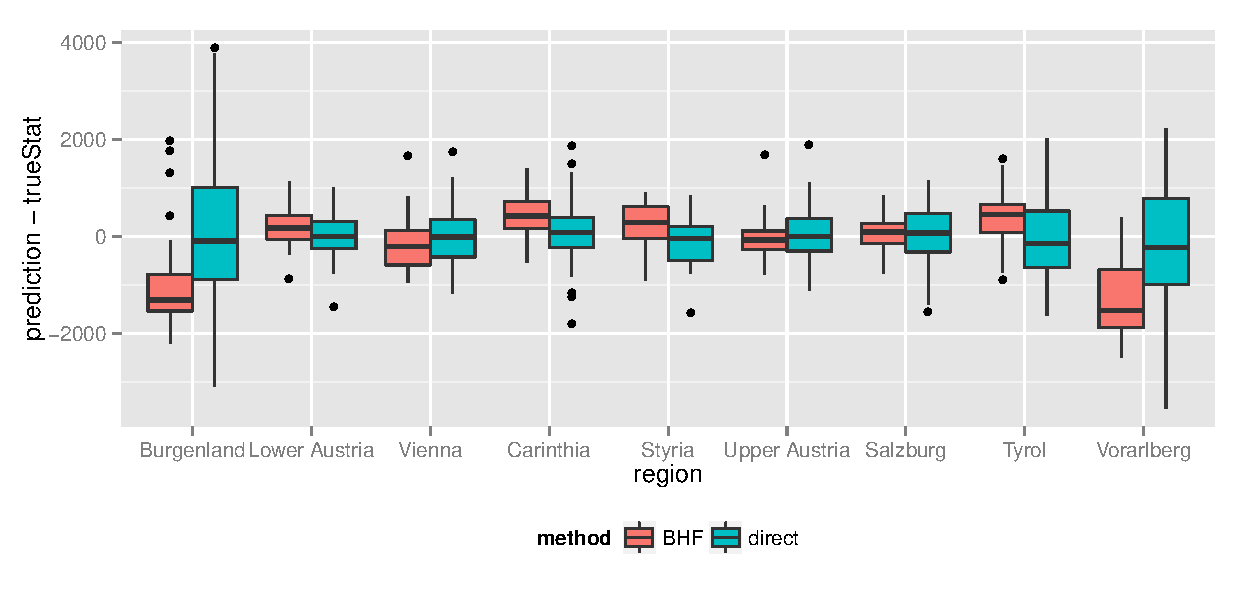
\includegraphics[width = \textwidth]{saeSim-designSimBIAS.pdf}
\caption{Monte-Carlo BIAS of direct vs. BHF predictor. 50 predictions for each region and estimation technique.}
\label{fig:dbBIAS}
\end{figure}



\begin{figure}[!h]
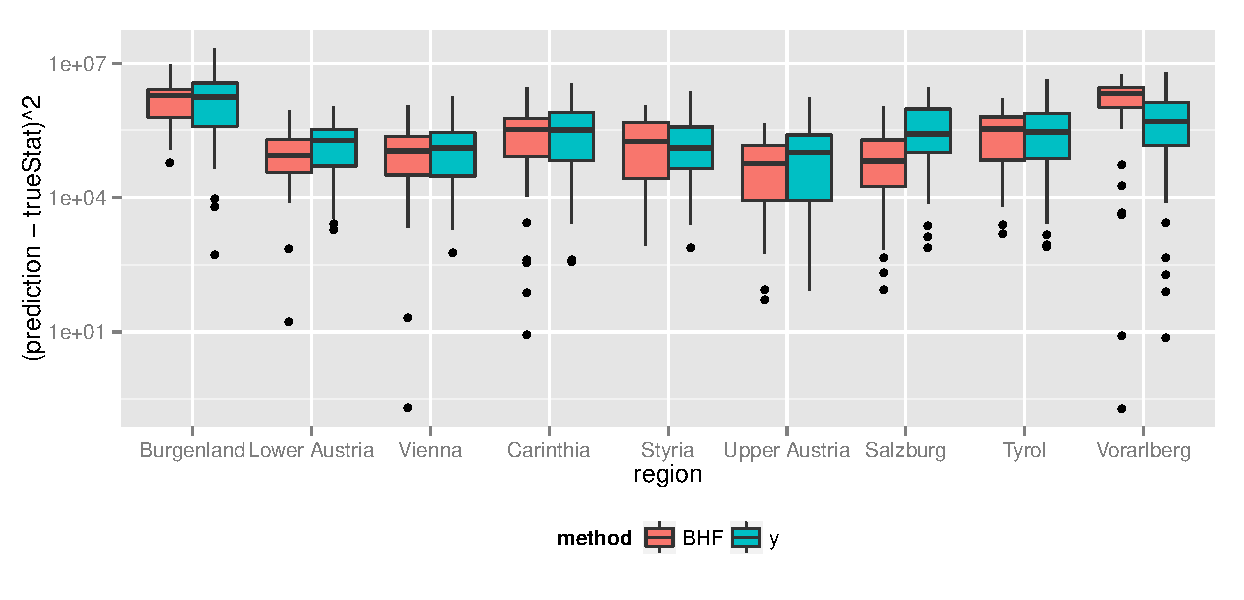
\includegraphics[width = \textwidth]{saeSim-designSimMSE.pdf}
\caption{Monte Carlo MSE of direct vs. BHF predictor. 50 predictions for each region and estimation technique.}
\label{fig:dbMSE}
\end{figure}
\clearpage

  
\section{Outlook}
\label{sec:outlook}
From our perspective, there is a need for sharing tools for data generation and simulation amongst the scientific community to guarantee the reproducibility of research. \proglang{saeSim} may provide an adequate framework for pursuing this aim in the field of small area estimation. By defining the steps of a simulation we may promote a reasonable way to communicate results in academic articles and during research. 

The package source is available on CRAN (\url{http://cran.r-project.org/web/packages/saeSim/}) and the repository for development on GitHub (\url{https://github.com/wahani/saeSim}). As GitHub allows to share and contribute source code using version-control, it is open for submissions. Apart from the availability of specific utility functions, we may promote and support the design of source code for simulation studies. One aspect is the design of simulations as processes of data. Furthermore, we encourage the definition of small and self contained components, i.e. functions. This reduces the lines of code necessary to be read in order to understand it's purpose. 

The package provides more features than introduced in this article. To mention is the support of outlier contaminated data. At this time only representative outliers (outlying observations in the population) are supported \citep[cf.][]{Cha86}. However, we plan to extend this feature to non-representative outliers (outliers are part of the sample but not the population). Furthermore, an interface to \proglang{R} random number generators is available. The user can also generate group effects as needed in mixed models. As the response is created by an \proglang{R} expression, any form of non-linearity in the relationship between response and auxiliary variables as well as error components can be modelled.

A more technical feature is a back-end for parallel computations which is a link to the \proglang{parallel} package in \proglang{R} \citep{r14}. Tools to process result data after the simulation, i.e. summaries or plotting methods, are avenues for further research. Already available are some simple plots for the simulation setups as well as a summary method to get information on the expected runtime and structure of the resulting data.

%\bibliographystyle{plainat}
\bibliography{saeSim}



\end{document}
